\section{Software struktur og funktionalitet}
Softwarens struktur er bygget op omkring to sensorer som måler temperatursvingninger mellem rummet og vandrøret. I dette afsnit vil de enkelte funktionerne i softwaren til fase 1 og 2 blive beskrevet. 
\begin{figure}[h!]
  \centering
  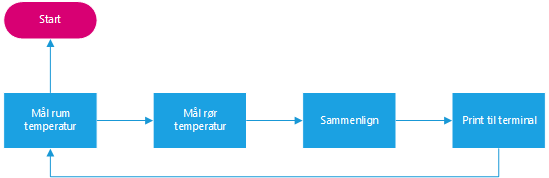
\includegraphics[width=0.5\textwidth]{figures/Fase1software.png}
  \caption{Fase 1 - Software flowchart.}
\end{figure}


\subsection{Mål rum temperatur}
\fxnote{skriv afsnit om hvordan rumtemperaturen bliver målt}
\subsection{Mål rør temperatur}
\fxnote{skriv afsnit om hvordan rørtemperaturen bliver målt}
\subsection{Sammenlign}
\fxnote{skriv afsnit om hvordan vi sammenligner temperaturerne, og hvorfor det er brugbart}
\subsection{Print til terminal}
\fxnote{skriv afsnit om hvordan data skal vises i terminalen, muligvis andre metoder?(gem i tekstfil, smid ind i mathcad for at få graf)}
\begin{figure}[h!]
  \centering
  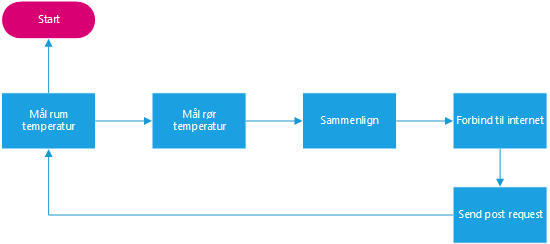
\includegraphics[width=1\textwidth]{figures/Fase2software.png}
  \caption{Fase 2 - Software flowchart.}
\end{figure}